% NeurIPS-style conference paper (5.5in x 9in text block, 10pt Times).
\documentclass[10pt]{article}

\usepackage[letterpaper, textwidth=6.0in, textheight=9.4in, top=0.8in, centering]{geometry}
\usepackage[utf8]{inputenc}
\usepackage[T1]{fontenc}
\usepackage{lmodern}
\usepackage{amsmath,amssymb}
\usepackage{booktabs}
\usepackage{graphicx}
\usepackage{xcolor}
\usepackage[authoryear,round]{natbib}
\usepackage[colorlinks=true,linkcolor=blue!60!black,citecolor=blue!60!black,urlcolor=blue!60!black]{hyperref}
\urlstyle{same}

\setlength{\parindent}{0pt}
\setlength{\parskip}{3pt}
\renewcommand{\topfraction}{0.94}
\renewcommand{\bottomfraction}{0.88}
\renewcommand{\textfraction}{0.05}
\setlength{\textfloatsep}{6pt plus 2pt minus 2pt}
\setlength{\floatsep}{5pt plus 2pt minus 2pt}
\setlength{\intextsep}{5pt plus 2pt minus 2pt}

\makeatletter
\renewcommand\section{\@startsection{section}{1}{0pt}{-9pt plus -2pt minus -1pt}{3pt plus 1pt}{\large\bfseries}}
\renewcommand\subsection{\@startsection{subsection}{2}{0pt}{-7pt plus -2pt minus -1pt}{2pt plus 1pt}{\normalsize\bfseries}}
\renewcommand\paragraph{\@startsection{paragraph}{4}{0pt}{4pt plus 1pt}{-0.6em}{\normalsize\bfseries}}
\makeatother

\newcommand{\code}[1]{\texttt{#1}}

\begin{document}

\begin{center}
  \rule{\linewidth}{2.0pt}\\[5pt]
  {\Large\bfseries Smooth Operator: Spectral Action Tokens and Learning\\Efficiency in Vision-Language-Action Adaptation\par}
  \vspace{4pt}
  \rule{\linewidth}{0.7pt}\\[6pt]
  {\normalsize\bfseries Isuru Suharshan (A0314895R)\quad\quad Vadiraj Rao (A0353463A)}\\[2pt]
  {\small School of Computing, National University of Singapore \quad
  \texttt{e1507191@u.nus.edu}, \texttt{vadiraj.anand.rao@u.nus.edu}}
\end{center}
\vspace{2pt}

\begin{abstract}
\noindent
Autoregressive Vision-Language-Action (VLA) models output robot motion as a sequence of discrete tokens, so the action tokenizer determines both the token count per chunk and how hard the policy's prediction problem is.
We test whether spectral representations of robot action chunks improve learning efficiency and open a path to token optimization when a pretrained $\pi_0$-FAST policy is adapted end to end on those tokens with LoRA.
Under a shared quantizer and grammar-constrained decoder, we compare localized spectral bases (Haar and other wavelets, which separate local averages from local changes and support per-chunk resolution) against global bases (the discrete cosine transform without byte-pair encoding, and discrete orthogonal Gram polynomials).
After ranking 26 wavelet schemes offline on LIBERO demonstrations, fixed Haar wavelets perform strongly on a single task, reaching 53/60 closed-loop successes at 2,000 updates versus 43/60 for DCT without BPE and 17/60 for matched FAST.
A scale-aware loss with soft bin labels and quantizer-step weighting follows naturally from wavelet orthonormality and matches plain cross-entropy on the single task (52/60).
When training scales to all 40 LIBERO tasks, however, wavelets fall behind DCT already at epoch 1: DCT reaches 77.0\% (308/400) versus 58.5\% (234/400) for plain Haar ($p = 2.1\times 10^{-13}$) and 53.0\% (212/400) for soft-weighted Haar.
A controlled synthetic test explains this reversal: when a smooth trajectory changes slightly, DCT changes 30\% of its tokens while Haar rewrites 69\%, turning multi-task adaptation into a learning-complexity problem rather than a reconstruction-error problem.
The same test ranks Gram orthogonal polynomials first (22\% of tokens changed).
Replacing DCT with Gram polynomials gives our best accuracy across all 40 tasks at both epochs: 81.2\% (325/400) at epoch 1 (91\% on LIBERO-Goal vs.\ 72\% for matched DCT, $p = 3.1\times 10^{-4}$) and 90.2\% (361/400) at epoch 2, significantly ahead of plain DCT (85.5\%, $p = 0.020$, with 81\% vs.\ 66\% on LIBERO-10, $p = 0.011$) and plain Haar (79.2\%, $p = 8.0\times 10^{-6}$).
Code and reproduction instructions: \url{https://github.com/isururajakaruna/vla-spectral-methods}.
\end{abstract}

\section{Introduction}
\label{sec:intro}

Autoregressive Vision-Language-Action (VLA) policies generate robot control commands the same way a language model writes text: one discrete token at a time, conditioned on camera images, robot state, and a task instruction.
Because robot actions are continuous vectors, an action tokenizer sits between the continuous motion and the discrete vocabulary.
That tokenizer shapes two things at once.
First, it sets the number of tokens per action chunk, which drives decoding latency and the number of sequential decisions the policy must get right.
Second, it defines the learning problem seen by the decoder: two nearby trajectories can share almost all their tokens in one basis and differ in almost every token in another.

Recent work such as FAST \citep{pertsch2025fast} applies a discrete cosine transform (DCT) followed by quantization and byte-pair encoding (BPE) to compress action chunks into short token streams.
Shorter streams decode faster, but they are not automatically easier to learn under a limited fine-tuning budget.
Because BPE merges several frequency coefficients into one symbol, a single wrong token can corrupt multiple time steps or leave the decoder with the wrong number of coefficients.
We ask a focused question: can spectral representations of action space improve learning efficiency and enable token optimization when a pretrained VLA is trained end to end on structured spectral tokens?

We test this across localized and global spectral bases on the LIBERO benchmark \citep{liu2023libero} using a frozen $\pi_0$-FAST backbone adapted with rank-16 LoRA \citep{hu2022lora}.
All structured variants share the same calibration rule, finite-state grammar mask, and training loop, so differences reflect the basis and loss rather than malformed outputs.
Our experiments follow a clear sequence:
(1) We rank 26 wavelet schemes offline on LIBERO chunks and show that fixed Haar wavelets learn faster than both matched FAST and DCT without BPE on a single manipulation task (53/60 at 2,000 updates).
(2) Motivated by wavelet orthonormality and a $30\times$ spread in quantizer steps across scales, we test soft target labels and step-weighted cross-entropy.
(3) Scaling to all 40 LIBERO tasks reverses the ranking already at epoch 1, with DCT at 77.0\% versus 58.5\% for plain Haar and 53.0\% for soft-weighted Haar.
(4) A synthetic perturbation test shows that small smooth path changes rewrite 69\% of Haar tokens versus 30\% of DCT tokens and 22\% of Gram polynomial tokens, pointing directly to orthogonal polynomials; trained from scratch, Gram polynomials reach 81.2\% at epoch 1 and 90.2\% at epoch 2, outperforming both plain DCT (85.5\%) and plain Haar (79.2\%).
Throughout the 40-task study, we compare all five variants across epochs 1 and 2 under identical schedules and evaluation episodes.
Code, checkpoints, and run commands are public at \url{https://github.com/isururajakaruna/vla-spectral-methods}.

\section{Related Work}
\label{sec:related}

\paragraph{Action chunking.}
Predicting a short block of future actions instead of a single step reduces compounding error in imitation learning.
ACT predicts continuous chunks with a conditional VAE \citep{zhao2023act}, and Diffusion Policy generates continuous trajectories by iterative denoising \citep{chi2023diffusion}.
Both show the value of modeling a chunk jointly, but they output continuous vectors rather than discrete tokens.
We keep the discrete autoregressive decoder of modern VLAs and study how the choice of spectral basis affects adaptation.

\paragraph{VLA adaptation and spectral tokenization.}
OpenVLA \citep{kim2024openvla} fine-tunes pretrained VLAs with LoRA \citep{hu2022lora} and per-step scalar binning, which wastes tokens when nearby steps are strongly correlated.
FAST \citep{pertsch2025fast} compresses chunks using a DCT, quantization, and BPE.
We evaluate both a matched FAST baseline and a DCT control without BPE under grammar-constrained decoding, separating the transform itself from compression artifacts.

\paragraph{Multiresolution wavelets and LIBERO.}
Wavelet transforms decompose signals into coarse trends and localized details across scales \citep{mallat1989wavelet}.
We apply classical Haar wavelets and discrete orthogonal polynomials to normalized action channels rather than claiming a new transform; our contribution is integrating them with structured gripper events, grammar masking, and closed-loop VLA evaluation on LIBERO's four task suites (Spatial, Object, Goal, and LIBERO-10) \citep{liu2023libero}.

\section{Rationale: Localized vs.\ Global Spectral Schemes}
\label{sec:rationale}

Every orthonormal $H \times H$ transform $T$ satisfies $\|T x_1 - T x_2\|_2 = \|x_1 - x_2\|_2$ for any two action chunks $x_1, x_2 \in \mathbb{R}^H$.
Before quantization, Haar wavelets, DCT-II, and orthogonal polynomials preserve distances identically and contain the exact same information.
What differs is how a trajectory and its small variations are distributed over the $H$ coefficient tokens, which is what an autoregressive model has to predict.

Two families offer distinct advantages for robot control:
\textbf{Localization-friendly bases (wavelets)} have compact support in time and split coarse averages from local changes.
Because manipulation chunks often combine smooth reaching with sudden contact or gripper switches, a localized basis can isolate abrupt events to a few time-aligned detail tokens and save tokens by dropping fine details on smooth segments (adaptive resolution).
\textbf{Global smooth bases (DCT and orthogonal polynomials)} span the entire chunk with global shape modes (offset, slope, curvature, higher oscillations).
Because 10-step robot motions are mostly smooth, energy concentrates into a few low-order coefficients whose semantic roles stay fixed across the whole chunk.
Because offline reconstruction error cannot predict which token distribution a transformer learns more easily, we test both families offline and in closed-loop simulation.

\section{Method}
\label{sec:method}

Figure~\ref{fig:pipeline} shows the shared adaptation pipeline.
The pretrained backbone, LoRA adapters, observations, and grammar mask stay fixed while we vary the spectral transform and loss.

\begin{figure}[t]
  \centering
  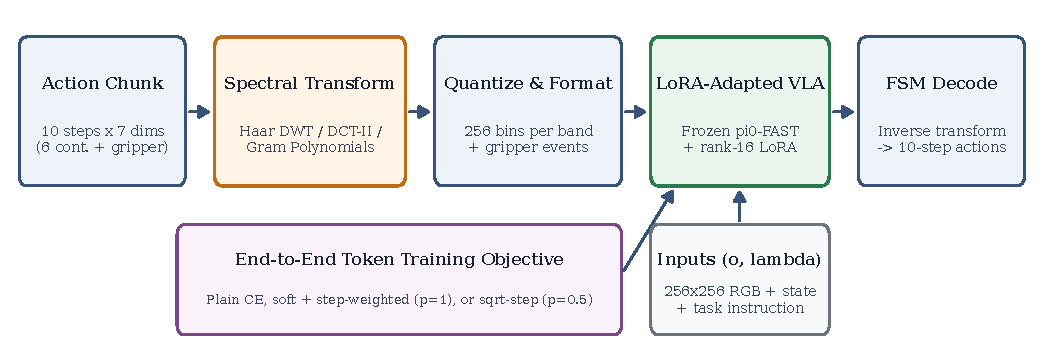
\includegraphics[width=0.92\linewidth]{figures/pipeline.pdf}
  \caption{Shared VLA adaptation pipeline. Continuous action channels pass through a spectral transform (Haar DWT, DCT-II, or Gram polynomials), band-wise quantization, and gripper event coding. The frozen $\pi_0$-FAST backbone is adapted end to end on the resulting tokens via rank-16 LoRA, and a finite-state machine guarantees valid streams at inference.}
  \label{fig:pipeline}
\end{figure}

\subsection{Action Normalization and Spectral Transforms}

An action chunk $A \in \mathbb{R}^{H \times 7}$ covers $H=10$ steps with six continuous end-effector deltas and one binary gripper channel.
Each continuous channel $d \in \{1,\dots,6\}$ is normalized using training-split mean $\mu_d$ and standard deviation $s_d$: $X_{t,d} = (A_{t,d} - \mu_d)/s_d$.
Each channel $x \in \mathbb{R}^H$ maps to coefficients $c = T x$, with reconstruction $\widehat{x} = S \widehat{c}$ ($S = T^{-1}$, and $S = T^\top$ when $T$ is orthonormal).

\paragraph{Haar wavelet transform (fixed and adaptive).}
On a power-of-two segment of length $L = 2^J$, Haar analysis recursively computes local averages and differences:
\begin{equation}
  a_j = \frac{x_{2j} + x_{2j+1}}{\sqrt{2}}, \qquad d_j = \frac{x_{2j} - x_{2j+1}}{\sqrt{2}}.
  \label{eq:haar}
\end{equation}
Keeping resolution $k \in \{0,\dots,J\}$ retains the $2^k$ coarsest coefficients per channel and zeroes finer details.
At $H=10$, fixed Haar uses the full-resolution plan $[(8,3),(2,1)]$.
To test token optimization, an adaptive dynamic-programming oracle picks segment lengths $L \in \{2,4,8\}$ and resolutions $k$ per training chunk by minimizing
\begin{equation}
  \ell(s,L,k) = \alpha \|X_{s:s+L} - \widehat{X}_{s:s+L}\|_F^2 + \beta \|D X_{s:s+L} - D \widehat{X}_{s:s+L}\|_F^2 + \gamma T(L,k),
  \label{eq:dp}
\end{equation}
where $D$ is the within-segment first difference, $T(L,k)$ is the token count, and $(\alpha,\beta,\gamma)=(1, 0.5, 0.005)$.
At inference the policy predicts the segment plan tokens itself.

\paragraph{DCT-II without BPE.}
As a clean control against FAST, we apply the orthonormal whole-window DCT-II to each 10-step channel:
\begin{equation}
  T^{\mathrm{DCT}}_{k,n} = \alpha_k \cos\!\left(\frac{\pi(2n+1)k}{2H}\right), \qquad
  \alpha_0 = \sqrt{\frac{1}{H}}, \quad \alpha_{k>0} = \sqrt{\frac{2}{H}}.
  \label{eq:dct}
\end{equation}
Coefficients are grouped into octave-like bands of sizes $(1, 1, 2, 6)$ (DC, first harmonic, frequencies 2--3, and 4--9) and emitted directly without BPE.

\paragraph{Discrete orthogonal (Gram) polynomials.}
Guided by our token-shift diagnosis (Section~\ref{sec:shift}), we build an orthonormal polynomial basis on the $H$ evenly spaced points $u_n = -1 + \frac{2n}{H-1}$ ($n=0,\dots,H-1$).
Evaluating Legendre polynomials $P_0,\dots,P_{H-1}$ at $\{u_n\}$ forms the Vandermonde matrix $V_{n,k} = P_k(u_n)$.
Taking the QR factorization $V = Q R$ (with signs fixed so $Q_{H-1,k} > 0$) gives
\begin{equation}
  T^{\mathrm{poly}} = Q^\top, \qquad S^{\mathrm{poly}} = Q.
  \label{eq:poly}
\end{equation}
QR mixes degree $k$ only with lower degrees, so row $k$ still represents the degree-$k$ motion component (offset, slope, curvature) while staying strictly orthonormal.
Coefficients are grouped by degree $(1, 1, 2, 6)$, matching DCT's bands, quantizer, grammar, and 64-token chunk length.
Starting QR from Chebyshev, Hermite, or monomial $u^k$ bases yields the exact same Gram basis up to signs.

\subsection{Quantization, Grammar Masking, and Scale-Aware Loss}

For each coefficient group and dimension, we fit center $m_i$ and step $\Delta_i > 0$ on training windows ($m_i = 0$ for detail groups) and quantize to 256 bins:
\begin{equation}
  b_i = \operatorname{clip}_{[0,255]}\!\left(\operatorname{round}\!\left(\frac{c_i - m_i}{\Delta_i}\right) + 127\right), \qquad
  \widehat{c}_i = m_i + (b_i - 127)\Delta_i.
  \label{eq:quant}
\end{equation}
Binary gripper values are serialized as an initial state plus transition time offsets, reproducing demonstrated switches exactly offline.
The local vocabulary has 302 symbols (256 bins plus structural and gripper tokens), and a finite-state machine masks illegal next tokens at inference so 0\% of generated chunks are malformed.
We adapt the frozen 3.47B-parameter $\pi_0$-FAST backbone (PaliGemma-3B + SigLIP) end to end on these tokens using rank-16 LoRA ($\alpha=16$) on all attention and MLP layers across 18 Gemma blocks plus trainable action-token rows (20.85M trainable parameters for all structured codecs; 23.81M for matched FAST).

Plain cross-entropy treats every token position and every wrong bin alike.
Yet for any orthonormal transform, Parseval's identity ties coefficient error directly to trajectory error:
\begin{equation}
  \|x - \widehat{x}\|_2^2 = \|c - \widehat{c}\|_2^2 = \sum_i \bigl((b_i - b_i^*)\Delta_i\bigr)^2.
  \label{eq:parseval}
\end{equation}
In our Haar codec, $\Delta_i$ spans roughly $30\times$ from the coarsest trends ($0.041$--$0.119$) to the finest details ($0.0037$--$0.0142$, half of all 60 coefficient tokens).
A one-bin miss on a coarse token therefore moves the robot roughly $30\times$ farther than a one-bin miss on a fine detail.
We therefore test soft target labels and step-based weights on coefficient positions $\mathcal{C}$:
\begin{align}
  q_i(b) &= \frac{\exp\!\left(-\frac{((b - b_i^*)\Delta_i)^2}{2\sigma^2}\right)}{\sum_{u=0}^{255} \exp\!\left(-\frac{((u - b_i^*)\Delta_i)^2}{2\sigma^2}\right)}, \qquad
  w_i = \frac{\Delta_i^p}{\operatorname{mean}_{j \in \mathcal{C}} \Delta_j^p}, \label{eq:softw} \\
  \mathcal{L} &= -\frac{1}{|\mathcal{M}|}\sum_{i \in \mathcal{M}} w_i \sum_b q_i(b)\log p_\theta(z_i=b \mid z_{<i}, o, \lambda). \label{eq:loss}
\end{align}
Non-coefficient tokens stay one-hot with weight 1.
We test plain cross-entropy ($p=0$, one-hot), full step weighting with soft labels ($p=1$, $\sigma=0.007$), and gentler square-root step weighting without soft labels ($p=0.5$, one-hot, giving weights in $[0.56, 2.82]$ for DCT and $[0.54, 2.76]$ for Gram polynomials versus $[0.25, 6.4]$ under $p=1$).

\section{Experiments and Results}
\label{sec:experiments}

\subsection{Protocol and Statistical Testing}

All experiments use the pinned \code{lerobot/libero} dataset with a seed-0 per-task 90/10 episode split; normalization and quantizers fit on training episodes only.
Training runs on one NVIDIA RTX A6000 (bf16, effective batch 16, peak lr $2\times 10^{-4}$, AdamW with $\beta=(0.9,0.95)$, grad clip 1.0).
The \textbf{single-task study} trains on LIBERO-Object task 0 (40 training episodes, 5,840 windows) over three seeds (0, 1, 2) on a 5,000-step cosine schedule stopped at 2,000 updates (100-step warmup), evaluated at steps 250, 500, 1,000, 1,500, and 2,000 on initial states 0--19 (60 episodes per point).
The \textbf{40-task study} trains on all 40 LIBERO tasks (1,525 training episodes, 232,282 windows, seed 0, 300-step warmup): epoch 1 runs to 14,500 updates under a 29,000-step cosine schedule, and epoch 2 resumes optimizer state to 29,000 updates under a 43,500-step cosine schedule (identical across all five models). Every checkpoint is evaluated on the exact same 400 episodes (10 initial states per task; suite limits 280 for Spatial/Object, 300 for Goal, 520 for LIBERO-10).
Because initial states are matched across models, we compare pairs with the two-sided exact McNemar test on discordant episodes (exploratory, uncorrected).

\subsection{Offline Wavelet Ranking}
\label{sec:wavelet_rank}

Before policy training, we ranked 26 single and mixed wavelet schemes offline on held-out LIBERO validation chunks (2,674 windows at $H=10$, 783 at $H=32$).
Each scheme was evaluated along its adaptive rate-distortion curve and ranked by the \textbf{tokens per chunk needed to match FAST's validation MSE} ($6.51\times 10^{-4}$ at $H=10$, $6.98\times 10^{-4}$ at $H=32$), averaged over both horizons (Table~\ref{tab:wavelets}; full list in Appendix~\ref{app:wavelets}).

\begin{table}[t]
  \centering
  \caption{Top offline wavelet schemes ranked by tokens/chunk needed to match FAST's validation MSE, averaged over $H=10$ and $H=32$ (coefficient tokens only). Full table in Appendix~\ref{app:wavelets}.}
  \label{tab:wavelets}
  \footnotesize
  \setlength{\tabcolsep}{4pt}
  \begin{tabular}{@{}clcccc@{}}
    \toprule
    Rank & Wavelet scheme (best mode) & $H=10$ & $H=32$ & vs.\ Haar & $H=10$ p99 err \\
    \midrule
    1 & \code{mix:sym4->haar} (sym.) & 60.5 & 157.7 & $-2.5\%$ & 0.181 \\
    2 & \code{mix:haar,haar->bior4.4} (per.) & 60.3 & 166.0 & $-0.2\%$ & 0.189 \\
    3 & \textbf{Haar} (periodization) & \textbf{60.3} & \textbf{166.7} & \textbf{0.0\%} & \textbf{0.184} \\
    6 & \code{bior1.3} (per.) & 60.5 & 168.2 & $+0.6\%$ & 0.185 \\
    9 & \code{db4} (per.) & 62.8 & 172.2 & $+3.7\%$ & 0.205 \\
    10 & \code{bior4.4} (per.) & 64.3 & 176.8 & $+6.3\%$ & 0.271 \\
    \bottomrule
  \end{tabular}
\end{table}

At $H=10$, none of the 25 alternatives beat Haar by 2\% or more: longer smooth filters (\code{db4}, \code{bior4.4}, \code{coif2}) cost 4--8\% more tokens due to boundary overhead on short 10-step windows.
Only at $H=32$ does \code{mix:sym4->haar} save 5.4\%.
We therefore chose Haar for our $H=10$ wavelet codec.
At full resolution on $H=10$, fixed Haar achieves MSE $1.45\times 10^{-4}$ with 69.1 tokens/chunk (adaptive Haar: $3.07\times 10^{-4}$ with 59.7 tokens) versus $6.51\times 10^{-4}$ with 24.9 tokens for FAST.

\subsection{Early Single-Task Results and Scale-Aware Soft Weighting}
\label{sec:single_task}

\begin{figure}[t]
  \centering
  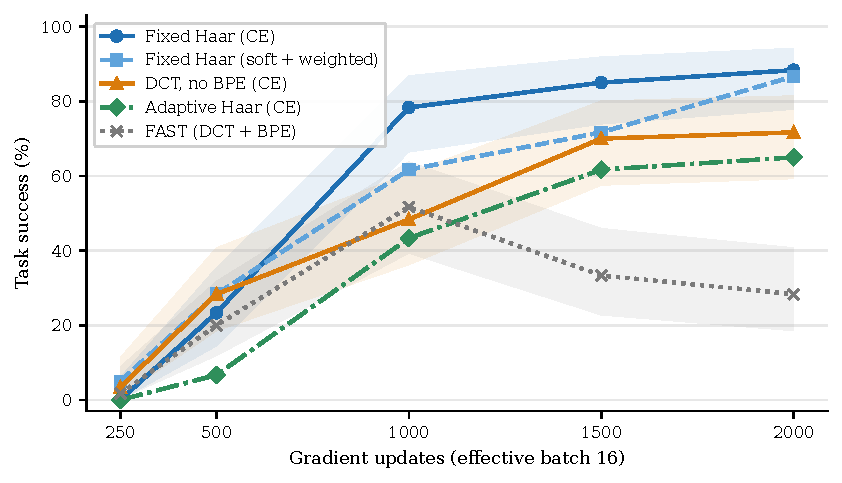
\includegraphics[width=0.66\linewidth]{figures/learning_curve.pdf}
  \caption{Closed-loop learning on LIBERO-Object task 0 (3 seeds $\times$ 20 initial states = 60 episodes/point; shading shows descriptive 95\% Wilson intervals). Fixed Haar reaches 78.3\% at 1,000 updates and 88.3\% at 2,000 updates.}
  \label{fig:lc}
\end{figure}

\begin{table}[t]
  \centering
  \caption{Single-task closed-loop results on LIBERO-Object task 0 at 2,000 updates (60 episodes across 3 seeds).}
  \label{tab:single}
  \footnotesize
  \setlength{\tabcolsep}{4pt}
  \begin{tabular}{@{}lccccc@{}}
    \toprule
    Variant & @1000 & @2000 & Seeds (0/1/2) & Tok/chunk & Lat.\ (ms) \\
    \midrule
    FAST (DCT + BPE) & 31/60 (51.7\%) & 17/60 (28.3\%) & 4/6/7 & 29.6 & 567 \\
    Adaptive Haar (CE) & 26/60 (43.3\%) & 39/60 (65.0\%) & 10/14/15 & 61.6 & 1,024 \\
    DCT, no BPE (CE) & 29/60 (48.3\%) & 43/60 (71.7\%) & 15/14/14 & 64.1 & 1,035 \\
    Fixed Haar (soft + wt) & 37/60 (61.7\%) & 52/60 (86.7\%) & 20/18/14 & 69.1 & 1,185 \\
    \textbf{Fixed Haar (CE)} & \textbf{47/60 (78.3\%)} & \textbf{53/60 (88.3\%)} & \textbf{16/18/19} & 69.1 & 1,134 \\
    \bottomrule
  \end{tabular}
\end{table}

Figure~\ref{fig:lc} and Table~\ref{tab:single} show that fixed Haar tokens learn quickly on the single task.
At 1,000 updates, fixed Haar reaches 47/60 (78.3\%), ahead of matched FAST (31/60, $p=0.002$) and DCT without BPE (29/60; 25 vs.\ 7 discordant episodes, $p=0.002$).
At 2,000 updates, fixed Haar reaches 53/60 (88.3\%), ahead of DCT without BPE (43/60; 15 vs.\ 5, $p=0.041$) and matched FAST (17/60; 37 vs.\ 1, $p=2.8\times 10^{-10}$).
Diagnostic logging shows that 89.0\% of FAST's generated chunks at 2,000 updates are malformed (wrong coefficient count, requiring fallback padding/truncation), whereas grammar-constrained DCT and Haar have 0\% malformed streams.
Adaptive Haar saves 7.5 tokens/chunk (61.6 vs.\ 69.1) but drops success to 39/60 because predicting variable plans adds discrete decisions that hurt policy learning.
Fixed Haar's higher accuracy also doubles decoding latency relative to FAST (1,134 ms vs.\ 567 ms per chunk).

Adding Parseval-motivated soft labels and step weighting ($p=1$, $\sigma=0.007$; Eq.~\ref{eq:loss}) to fixed Haar yields 52/60 at 2,000 updates, statistically tied with plain cross-entropy (53/60; 6 vs.\ 7 discordant, $p=1.0$).
Seed 0 reached 20/20 (the only perfect seed in the study), though seeds 1 and 2 scored 18/20 and 14/20 and mid-training convergence at 1,000--1,500 updates was slightly slower because soft targets dilute exact-bin supervision.
Because the objective is well motivated by Eq.~(\ref{eq:parseval}) and matched plain cross-entropy at 2,000 updates, we carried soft-weighted Haar into 40-task training alongside a plain Haar control.

\subsection{Scaling to 40 Tasks: Wavelets Lag Behind DCT at Epoch 1}
\label{sec:scaling}

When training scales to all 40 LIBERO tasks (14,500 updates = 1 epoch), the single-task ranking reverses immediately (first three rows of Table~\ref{tab:epoch1}).
Plain DCT without BPE reaches \textbf{77.0\%} (308/400), beating plain Haar at \textbf{58.5\%} (234/400) by 18.5 percentage points (91 vs.\ 17 discordant episodes, $p = 2.1\times 10^{-13}$).
DCT leads plain Haar on every suite: Spatial (89\% vs.\ 70\%), Object (92\% vs.\ 84\%), Goal (76\% vs.\ 50\%), and LIBERO-10 (51\% vs.\ 30\%).
Soft labels plus full step weighting do not help Haar at scale: soft-weighted Haar scores \textbf{53.0\%} (212/400), slightly below plain Haar (74 vs.\ 52 discordant, $p=0.061$) and 24 points below DCT ($p=2.6\times 10^{-16}$).
Because plain DCT and plain Haar share the same data, LoRA adapters, schedule, quantizer design, and grammar mask, the 18.5-point gap points directly to the basis representation.

\subsection{Diagnosis: Token Shift Under Small Trajectory Changes}
\label{sec:shift}

We hypothesized that multi-task adaptation exposes a \emph{learning-complexity} bottleneck: across 40 tasks, a policy must generalize over families of similar motions that differ by a small shift in slope, offset, curvature, or timing.
If a small path change alters only a few tokens in DCT but alters most tokens in Haar, then Haar gives the decoder a much harder symbol-prediction problem.

To isolate this effect cleanly without dataset confounds, we ran a synthetic perturbation study across 18 transforms (wavelets, Fourier-family bases, orthogonal polynomials, Walsh-Hadamard, learned PCA, and raw samples).
We generated 400 random smooth paths (random sums of a cosine, cubic polynomial, Gaussian bump, and $\tanh$ step, normalized to peak-to-peak range 2) and applied 9 visible edits to each: slope up, slope down, constant offset, growing amplitude, decaying amplitude, added curvature, a local bump, a 6\% time delay, and a time warp ($t^{1.25}$).
Every transform $T$ was held to the exact same reconstruction accuracy by setting each coefficient's quantizer step to $q_i = s / \|S_{:,i}\|_2$ with $s = 0.02$ (so rounding any coefficient by one bin adds the same trajectory error in every basis).
We then measured the share of quantized tokens that change after an edit.

\begin{figure}[t]
  \centering
  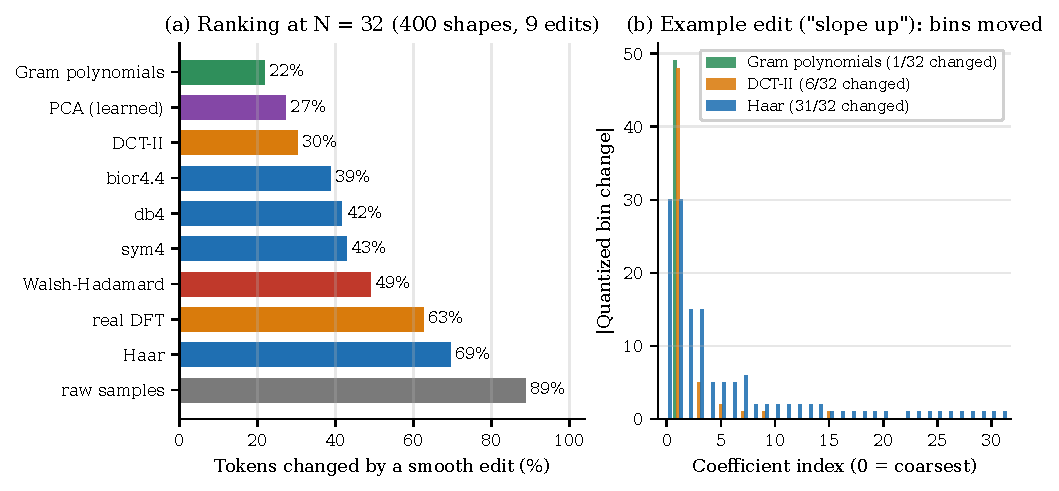
\includegraphics[width=0.86\linewidth]{figures/token_shift.pdf}
  \caption{Synthetic token-shift study (400 random smooth paths, 9 edits, equal-accuracy quantizer $s=0.02$). (a) Mean share of tokens changed per edit at $N=32$ (10 of 18 bases shown; full list in Appendix~\ref{app:shift}). Gram polynomials rank first (22\%), DCT-II third (30\%), and Haar 17th (69\%). (b) Bin changes for one ``slope up'' edit: Gram polynomials move 1/32 tokens, DCT moves 6/32, and Haar spreads changes across 31/32 tokens.}
  \label{fig:shift}
\end{figure}

Figure~\ref{fig:shift} separates the bases cleanly.
At $N=32$, DCT-II changes 30\% of tokens per edit, learned PCA changes 27\%, and \textbf{Gram orthogonal polynomials rank first of all 18 transforms at 22\%}.
By contrast, \textbf{Haar changes 69\% of tokens} (17th of 18, ahead only of raw samples at 89\%), and even smoother wavelets (\code{bior4.4} 39\%, \code{db4} 42\%, \code{sym4} 43\%) trail DCT and polynomials.
Panel (b) shows why: adding a simple linear slope moves 1 of 32 tokens in Gram polynomials (exact degree-1 mode) and 6 of 32 in DCT, but ripples into 31 of 32 tokens in Haar as small $\pm 1$ or $\pm 2$ bin flips across fine detail slots.
Two companion checks (Appendix~\ref{app:shift}) reinforce this mechanism: different edits of the same path overlap on fewer token positions under Gram polynomials (28\%) and DCT (35\%) than under Haar (51\%), while the \emph{top 3\% strongest coefficients} shift by almost the same amount in every orthonormal basis (26.7--32.7 bins at $N=64$).
Thus the coarse coefficients move similarly everywhere; the difference is in the weak coefficients, which DCT and polynomials leave quiet while Haar constantly rewrites.

\subsection{Polynomial Hypothesis and Payoff Across Epochs 1 and 2}
\label{sec:payoff}

Before training a polynomial policy, we compared polynomial and spline families at the actual training horizon $H=10$ (Appendix~\ref{app:poly}).
QR-orthonormalizing Legendre, Chebyshev, Hermite, or monomial $t^k$ bases on evenly spaced points yields the exact same Gram basis (verified to $10^{-6}$), while Chebyshev polynomials on Chebyshev nodes equal DCT-II.
Raw non-orthogonal polynomial bases are badly conditioned (condition number 819 for Hermite and 3,660 for monomials already at $H=10$), and local cubic B-splines behave like raw samples (92\% of tokens changed).
At $H=10$, Gram polynomials change 51\% of tokens per edit versus 59\% for DCT-II and 65\% for the whole-window \code{sym4->haar} codec, while matching DCT's offline LIBERO validation MSE at the exact same 64 tokens/chunk ($1.64\times 10^{-4}$ vs.\ $1.65\times 10^{-4}$).

We trained the Gram polynomial tokenizer (\code{poly\_fixed}) from scratch for two epochs on all 40 LIBERO tasks with gentler square-root step weighting ($p=0.5$, no soft labels), alongside a matched square-root-weighted DCT run from scratch so the transform comparison holds the loss constant.
Table~\ref{tab:epoch1} and Figure~\ref{fig:epoch1} present all five models across epochs 1 and 2 on the same 400 episodes.

\begin{table}[t]
  \centering
  \caption{Full 40-task LIBERO results at \textbf{epoch 1} (14,500 updates) and \textbf{epoch 2} (29,000 updates), all seed 0 on the exact same 400 episodes (100 per suite). Two-sided exact McNemar $p$-values compare each model with plain Haar and plain DCT at the same epoch.}
  \label{tab:epoch1}
  \scriptsize
  \setlength{\tabcolsep}{3.2pt}
  \begin{tabular}{@{}lccccccc@{}}
    \toprule
    Model & Spatial & Object & Goal & LIB-10 & Overall & vs.\ Haar & vs.\ DCT \\
    \midrule
    \multicolumn{8}{@{}l}{\textit{Epoch 1 (14,500 updates)}} \\
    Haar (soft + wt, $p=1$) & 57\% & 70\% & 63\% & 22\% & 53.0\% (212) & $p=0.061$ & $2.6\mathrm{e}{-16}$ \\
    Haar (plain CE) & 70\% & 84\% & 50\% & 30\% & 58.5\% (234) & -- & $2.1\mathrm{e}{-13}$ \\
    DCT, no BPE (plain CE) & 89\% & 92\% & 76\% & 51\% & 77.0\% (308) & $2.1\mathrm{e}{-13}$ & -- \\
    DCT, no BPE ($\sqrt{\text{step}}$, $p=0.5$) & 90\% & 95\% & 72\% & 61\% & 79.5\% (318) & $2.2\mathrm{e}{-14}$ & $p=0.353$ \\
    \textbf{Gram poly ($\sqrt{\text{step}}$, $p=0.5$)} & 87\% & 91\% & \textbf{91\%} & 56\% & \textbf{81.2\% (325)} & $1.8\mathrm{e}{-16}$ & $p=0.100$ \\
    \midrule
    \multicolumn{8}{@{}l}{\textit{Epoch 2 (29,000 updates)}} \\
    Haar (soft + wt, $p=1$) & 77\% & 86\% & 67\% & 46\% & 69.0\% (276) & $1.1\mathrm{e}{-4}$ & $7.7\mathrm{e}{-10}$ \\
    Haar (plain CE) & 94\% & 89\% & 80\% & 54\% & 79.2\% (317) & -- & $p=0.006$ \\
    DCT, no BPE (plain CE) & 92\% & 97\% & 87\% & 66\% & 85.5\% (342) & $p=0.006$ & -- \\
    DCT, no BPE ($\sqrt{\text{step}}$, $p=0.5$) & \textbf{96\%} & \textbf{99\%} & \textbf{88\%} & 70\% & 88.2\% (353) & $5.6\mathrm{e}{-5}$ & $p=0.228$ \\
    \textbf{Gram poly ($\sqrt{\text{step}}$, $p=0.5$)} & 93\% & \textbf{99\%} & \textbf{88\%} & \textbf{81\%} & \textbf{90.2\% (361)} & $8.0\mathrm{e}{-6}$ & \textbf{$p=0.020$} \\
    \bottomrule
  \end{tabular}
\end{table}

\begin{figure}[t]
  \centering
  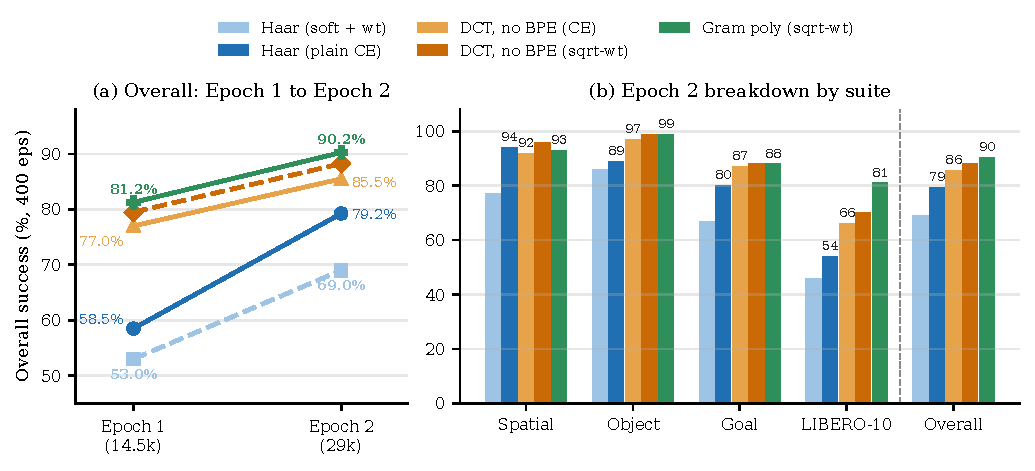
\includegraphics[width=0.88\linewidth]{figures/epoch1_suites.pdf}
  \caption{Full 40-task LIBERO closed-loop success across all five schemes (400 episodes/model). (a) Overall progression from epoch 1 to epoch 2: the ordering matches the synthetic token-shift ranking at both epochs. (b) Epoch-2 suite breakdown: Gram polynomials reach 90.2\% overall and 81\% on long-horizon LIBERO-10 (+15 points over plain DCT, $p=0.011$).}
  \label{fig:epoch1}
\end{figure}

The polynomial hypothesis paid off at both epochs:
\begin{itemize}\setlength{\itemsep}{1.2pt}\setlength{\parskip}{0pt}\setlength{\topsep}{2pt}
  \item \textbf{Best accuracy at epoch 1 and epoch 2.} Gram polynomials reach \textbf{81.2\%} at epoch 1 (beating plain Haar by 22.7 points, $p=1.8\times 10^{-16}$, and leading plain DCT by 4.2 points, $p=0.100$) and climb to \textbf{90.2\%} (361/400) at epoch 2. At epoch 2, Gram polynomials significantly beat both plain Haar (+11.0 points, 70 vs.\ 26 discordant, $p=8.0\times 10^{-6}$) and plain DCT (+4.7 points, 40 vs.\ 21 discordant, $p=0.020$), and lead matched $\sqrt{\text{step}}$-weighted DCT by 2.0 points (40 vs.\ 32 discordant, $p=0.410$).
  \item \textbf{Monotonic match with token shift at both epochs.} At epoch 1 and epoch 2 alike, closed-loop success rises monotonically as synthetic token shift falls: Haar (69\% shifted $\to$ 58.5\% / 79.2\%), DCT (30\% $\to$ 77.0\% / 85.5\% plain; 79.5\% / 88.2\% $\sqrt{\text{step}}$), and Gram polynomials (22\% $\to$ 81.2\% / 90.2\%).
  \item \textbf{Early Goal advantage, epoch-2 LIBERO-10 breakout.} At epoch 1, Gram polynomials lead strongly on LIBERO-Goal (91\% vs.\ 72\% for matched DCT, $p=3.1\times 10^{-4}$). By epoch 2, Spatial, Object, and Goal saturate near 88--99\% across global bases, and Gram polynomials separate on the hardest long-horizon suite, jumping 25 points on \textbf{LIBERO-10} to \textbf{81\%} versus 66\% for plain DCT (23 vs.\ 8 discordant, $p=0.011$), 70\% for matched $\sqrt{\text{step}}$-weighted DCT (24 vs.\ 13, $p=0.099$), and 54\% for plain Haar ($p=1.1\times 10^{-4}$).
  \item \textbf{Gentle weighting helps without slowing learning.} Full step weighting plus soft labels ($p=1$) hurt Haar at both epochs (69.0\% vs.\ 79.2\% at epoch 2, $p=1.1\times 10^{-4}$). By contrast, gentler square-root weighting ($p=0.5$, one-hot) kept DCT slightly ahead of plain DCT at both epoch 1 (+2.5 points, $p=0.35$) and epoch 2 (+2.7 points, $p=0.23$).
\end{itemize}

\section{Discussion, Limitations, and Conclusion}
\label{sec:conclusion}

\paragraph{Limitations.}
First, every 40-task model uses one training seed and 10 initial states per task (roughly $\pm 4$ percentage-point 95\% binomial width, versus 50 episodes per task in standard LIBERO evaluations).
Thus, while the gap between global bases and Haar ($p < 10^{-5}$ at both epochs), the epoch-1 Goal gain ($p = 3.1\times 10^{-4}$), and the epoch-2 gains of Gram polynomials over plain DCT overall ($p=0.020$) and on LIBERO-10 ($p=0.011$) are statistically strong, the 2.0-point margin of Gram polynomials over matched $\sqrt{\text{step}}$-weighted DCT at epoch 2 is not statistically significant ($p=0.41$) and needs multi-seed validation.
Second, our synthetic paths are smooth by construction; real chunks with hard contacts may narrow the advantage of global bases, so the token-shift study is an explanation consistent with the data rather than a causal proof.
Third, structured spectral tokens eliminate FAST's malformed streams and improve learning efficiency, but at 64--69 tokens/chunk they roughly double decoding latency relative to FAST's 30-token BPE stream, and adaptive Haar's 11\% token reduction hurt single-task success.
Finally, our transform matrix is fixed rather than learned jointly with the policy, and longer multi-epoch training is ongoing.

\paragraph{Conclusion.}
We studied how spectral representations of action space affect end-to-end learning efficiency and token structure when adapting a pretrained VLA with LoRA.
Offline reconstruction fidelity and single-task success did not predict multi-task learnability: Haar wavelets ranked near the top offline and won on a single task (53/60 vs.\ 43/60 for DCT and 17/60 for FAST), yet trailed DCT by 18.5 points at 40-task epoch 1 (58.5\% vs.\ 77.0\%) and 6.3 points at epoch 2 (79.2\% vs.\ 85.5\%).
A synthetic token-shift test revealed that small smooth trajectory changes rewrite 69\% of Haar tokens versus 30\% of DCT tokens and 22\% of Gram polynomial tokens, framing multi-task adaptation as a learning-complexity problem.
Guided by that ranking, Gram orthogonal polynomials achieved our best accuracy across all 40 tasks at both epoch 1 (81.2\%, 91\% on Goal) and epoch 2 (90.2\%, 81\% on LIBERO-10) at the exact same token count and reconstruction accuracy as DCT.
Two natural next steps follow: learning an orthonormal spectral basis end to end (since learned PCA ranked second in our token-shift study at 27\%), and compressing global polynomial streams via degree truncation or structured coding to recover FAST-level decoding speed without losing learning efficiency.

\clearpage
\bibliographystyle{plainnat}
\begin{thebibliography}{9}

\bibitem[Chi et~al.(2023)]{chi2023diffusion}
Cheng Chi, Siyuan Feng, Yilun Du, Zhenjia Xu, Eric Cousineau, Benjamin Burchfiel, and Shuran Song.
Diffusion Policy: Visuomotor Policy Learning via Action Diffusion.
\emph{Robotics: Science and Systems (RSS)}, 2023.
\url{https://arxiv.org/abs/2303.04137}.

\bibitem[Hu et~al.(2022)]{hu2022lora}
Edward J. Hu, Yelong Shen, Phillip Wallis, Zeyuan Allen-Zhu, Yuanzhi Li, Shean Wang, Lu Wang, and Weizhu Chen.
LoRA: Low-Rank Adaptation of Large Language Models.
\emph{International Conference on Learning Representations (ICLR)}, 2022.
\url{https://arxiv.org/abs/2106.09685}.

\bibitem[Kim et~al.(2024)]{kim2024openvla}
Moo Jin Kim, Karl Pertsch, Siddharth Karamcheti, Ted Xiao, Ashwin Balakrishna, Suraj Nair, Rafael Rafailov, Ethan Foster, Grace Lam, Pannag Sanketi, Quan Vuong, Thomas Kollar, Benjamin Burchfiel, Russ Tedrake, Dorsa Sadigh, Sergey Levine, Percy Liang, and Chelsea Finn.
OpenVLA: An Open-Source Vision-Language-Action Model.
\emph{arXiv preprint arXiv:2406.09246}, 2024.
\url{https://arxiv.org/abs/2406.09246}.

\bibitem[Liu et~al.(2023)]{liu2023libero}
Bo Liu, Yifeng Zhu, Chongkai Gao, Yihao Feng, Qiang Liu, Yuke Zhu, and Peter Stone.
LIBERO: Benchmarking Knowledge Transfer for Lifelong Robot Learning.
\emph{Advances in Neural Information Processing Systems (NeurIPS)}, 36, Datasets and Benchmarks Track, 2023.
\url{https://arxiv.org/abs/2306.03310}.

\bibitem[Mallat(1989)]{mallat1989wavelet}
St\'ephane G. Mallat.
A Theory for Multiresolution Signal Decomposition: The Wavelet Representation.
\emph{IEEE Transactions on Pattern Analysis and Machine Intelligence}, 11(7):674--693, 1989.

\bibitem[Pertsch et~al.(2025)]{pertsch2025fast}
Karl Pertsch, Kyle Stachowicz, Brian Ichter, Danny Driess, Suraj Nair, Quan Vuong, Oier Mees, Chelsea Finn, and Sergey Levine.
FAST: Efficient Action Tokenization for Vision-Language-Action Models.
\emph{arXiv preprint arXiv:2501.09747}, 2025.
\url{https://arxiv.org/abs/2501.09747}.

\bibitem[Zhao et~al.(2023)]{zhao2023act}
Tony Z. Zhao, Vikash Kumar, Sergey Levine, and Chelsea Finn.
Learning Fine-Grained Bimanual Manipulation with Low-Cost Hardware.
\emph{Robotics: Science and Systems (RSS)}, 2023.
\url{https://arxiv.org/abs/2304.13705}.

\end{thebibliography}

\clearpage
\appendix

\section{Implementation, Hyperparameters, and Reproduction}
\label{app:impl}

All models adapt \code{lerobot/pi0fast-base} (PaliGemma-3B + SigLIP, frozen) with rank-16 LoRA ($\alpha=16$) on \code{q/k/v/o} and \code{gate/up/down} projections in all 18 Gemma layers (126 linear layers) plus trainable residual rows for action tokens in the embedding and LM head (20.85M trainable parameters for structured codecs, 23.81M for matched FAST).
Shared training settings: NVIDIA RTX A6000 (48 GB, bf16), micro-batch 8 $\times$ gradient accumulation 2 = effective batch 16, peak learning rate $2\times 10^{-4}$, AdamW ($\beta_1=0.9$, $\beta_2=0.95$, weight decay 0), gradient-norm clip 1.0, $\approx 3.21$--$3.27$ s/step ($\approx 13$ hours per 14,500-step full-LIBERO epoch, plus $\approx 2.5$ hours for the 400-episode closed-loop evaluation).
Token stream grammar for whole-window DCT and Gram polynomials: \code{<RES\_k>}, 60 quantized coefficient tokens in row-major order (band, dimension), gripper initial state, gripper transition offsets, \code{<G\_END>}, \code{<A\_END>} ($\approx 64.1$ tokens/chunk).
Quantizer step ranges across the 60 coefficient positions: $[0.0070, 0.1793]$ for DCT and $[0.0068, 0.1793]$ for Gram polynomials.

Code and adapter weights (via Git LFS) are at \url{https://github.com/isururajakaruna/vla-spectral-methods}.
To reproduce the offline studies and polynomial training from \code{experiment/adaptive\_dwt\_vla/}:
{\scriptsize
\begin{verbatim}
python scripts/wavelet_selection.py
python scripts/transform_shift_analysis.py
python scripts/transform_polynomial_variants.py
python scripts/train.py --variant poly_fixed --weight-power 0.5 \
  --name full_s0_poly_fixed_sqrtw --seed 0 --tasks $(seq 0 39) \
  --horizon 10 --steps 29000 --stop-at 14500
\end{verbatim}
}

\section{Extended Offline Wavelet Ranking}
\label{app:wavelets}

Table~\ref{tab:wavelets_full} lists the top 15 of 26 tested wavelet schemes (excluding \code{dmey}, whose truncated FIR filter did not achieve $10^{-6}$ perfect reconstruction).
Mixed transforms apply a different wavelet per decomposition level (finest level first).
Symmetric boundary mode adds edge coefficients that inflate $H=10$ token counts (median $+104\%$ vs.\ Haar), so periodization mode wins for almost all single wavelets.

\begin{table}[ht]
  \centering
  \caption{Top 15 wavelet schemes from \code{scripts/wavelet\_selection.py}, ranked by mean token count relative to Haar at FAST's validation MSE ($6.51\times 10^{-4}$ at $H=10$, $6.98\times 10^{-4}$ at $H=32$).}
  \label{tab:wavelets_full}
  \scriptsize
  \setlength{\tabcolsep}{3.5pt}
  \begin{tabular}{@{}clccccc@{}}
    \toprule
    Rank & Transform & Taps & $H=10$ (mode) & $H=32$ (mode) & vs.\ Haar & Edge MSE \\
    \midrule
    1 & \code{mix:sym4->haar} & 8, 2 & 60.5 (sym.) & 157.7 (sym.) & $-2.5\%$ & $6.3\times 10^{-4}$ \\
    2 & \code{mix:haar,haar->bior4.4} & 2, 2, 10 & 60.3 (per.) & 166.0 (per.) & $-0.2\%$ & $6.3\times 10^{-4}$ \\
    3 & \code{haar} & 2 & 60.3 (per.) & 166.7 (per.) & $+0.0\%$ & $5.8\times 10^{-4}$ \\
    4 & \code{mix:haar->bior2.2} & 2, 6 & 60.4 (per.) & 166.3 (per.) & $+0.0\%$ & $7.1\times 10^{-4}$ \\
    5 & \code{mix:haar->db2->db4} & 2, 4, 8 & 60.4 (per.) & 166.8 (per.) & $+0.2\%$ & $6.9\times 10^{-4}$ \\
    6 & \code{bior1.3} & 6 & 60.5 (per.) & 168.2 (per.) & $+0.6\%$ & $5.5\times 10^{-4}$ \\
    7 & \code{mix:haar->sym4} & 2, 8 & 61.2 (per.) & 166.6 (per.) & $+0.7\%$ & $7.1\times 10^{-4}$ \\
    8 & \code{sym5} & 10 & 62.7 (per.) & 169.6 (per.) & $+2.9\%$ & $1.3\times 10^{-3}$ \\
    9 & \code{db4} & 8 & 62.8 (per.) & 172.2 (per.) & $+3.7\%$ & $1.2\times 10^{-3}$ \\
    10 & \code{bior4.4} & 10 & 64.3 (per.) & 176.8 (per.) & $+6.3\%$ & $1.4\times 10^{-3}$ \\
    11 & \code{bior6.8} & 18 & 64.5 (per.) & 176.5 (per.) & $+6.4\%$ & $1.4\times 10^{-3}$ \\
    12 & \code{coif3} & 18 & 64.9 (per.) & 176.9 (per.) & $+6.9\%$ & $1.6\times 10^{-3}$ \\
    13 & \code{coif2} & 12 & 64.8 (per.) & 177.3 (per.) & $+7.0\%$ & $1.6\times 10^{-3}$ \\
    14 & \code{bior2.2} & 6 & 64.7 (per.) & 177.9 (per.) & $+7.0\%$ & $1.2\times 10^{-3}$ \\
    15 & \code{bior2.4} & 10 & 65.0 (per.) & 177.7 (per.) & $+7.2\%$ & $1.1\times 10^{-3}$ \\
    \bottomrule
  \end{tabular}
\end{table}

\section{Synthetic Token-Shift, Fingerprint, and Top-3\% Studies}
\label{app:shift}

Table~\ref{tab:shift_full} reports all 18 transforms from the synthetic perturbation study at $N=32$ ($s=0.02$), together with companion metrics from our fingerprint and top-3\% coefficient analyses:
\emph{Tokens changed} is the mean share of the 32 tokens whose bin moves after one of the 9 edits;
\emph{Edit overlap} is the mean Jaccard overlap of moved token positions between two different edits of the same shape (lower means different edits touch more distinct tokens);
\emph{Top-3\% bin shift} ($N=64$, $k=2$) is the mean $|\Delta \text{bin}|$ of the two largest coefficients.
All orthonormal bases cluster tightly between 26.7 and 32.7 bins on the top-3\% shift, confirming that the difference between bases lies in the many weak coefficients rather than the strongest ones.

\begin{table}[ht]
  \centering
  \caption{All 18 transforms ranked by mean tokens changed at $N=32$ ($s=0.02$), with edit-to-edit Jaccard overlap ($N=32$) and top-3\% bin shift ($N=64$, $k=2$).}
  \label{tab:shift_full}
  \scriptsize
  \setlength{\tabcolsep}{4pt}
  \begin{tabular}{@{}cllccc@{}}
    \toprule
    Rank & Transform & Family & Changed ($N=32$) & Overlap ($N=32$) & Top-3\% ($N=64$) \\
    \midrule
    1 & Gram polynomials & polynomial & 22\% & 28\% & 26.7 bins \\
    2 & PCA (learned) & data-driven & 27\% & 64\% & 32.7 bins \\
    3 & DCT-II & Fourier & 30\% & 35\% & 29.2 bins \\
    4 & \code{bior4.4} & wavelet & 39\% & 52\% & 26.7 bins \\
    5 & \code{coif2} & wavelet & 42\% & 53\% & 27.8 bins \\
    6 & \code{bior2.2} & wavelet & 42\% & 44\% & 28.2 bins \\
    7 & \code{db4} & wavelet & 42\% & 53\% & 29.9 bins \\
    8 & \code{sym6} & wavelet & 42\% & 52\% & 27.9 bins \\
    9 & \code{sym4} & wavelet & 43\% & 51\% & 28.3 bins \\
    10 & \code{db6} & wavelet & 43\% & 56\% & 27.4 bins \\
    11 & \code{coif1} & wavelet & 48\% & 45\% & 26.8 bins \\
    12 & \code{db2} & wavelet & 48\% & 45\% & 27.9 bins \\
    13 & \code{dmey} & wavelet & 49\% & 53\% & 27.6 bins \\
    14 & Walsh-Hadamard & other & 49\% & 31\% & 26.8 bins \\
    15 & DST-II & Fourier & 60\% & 43\% & 30.2 bins \\
    16 & real DFT & Fourier & 63\% & 46\% & 28.1 bins \\
    17 & Haar & wavelet & 69\% & 51\% & 30.0 bins \\
    18 & raw samples & baseline & 89\% & 79\% & 7.6 bins \\
    \bottomrule
  \end{tabular}
\end{table}

\section{Polynomial and Spline Variants at the Training Horizon (H = 10)}
\label{app:poly}

Table~\ref{tab:poly_variants} summarizes the basis comparison at $H=10$ (400 shapes, 9 edits, equal-accuracy quantizer $s=0.02$).
Non-orthogonal polynomial families suffer from conditioning growth and noise sensitivity (subtle edit identification under white jitter drops from 78\% for Gram polynomials to 47\% for raw Chebyshev/Legendre and 25\% for monomials).
Local B-splines behave like raw samples and move over 90\% of tokens per edit.

\begin{table}[ht]
  \centering
  \caption{Polynomial and spline bases at the training horizon $H=10$ compared with DCT-II and the trained \code{sym4->haar} wavelet codec.}
  \label{tab:poly_variants}
  \scriptsize
  \setlength{\tabcolsep}{3.5pt}
  \begin{tabular}{@{}lccccc@{}}
    \toprule
    Basis ($H=10$) & Cond. & Changed & Overlap & Top-3\% & Subtle ID (sm./wh.) \\
    \midrule
    \textbf{Gram polynomials (ortho.)} & \textbf{1} & \textbf{51\%} & \textbf{33\%} & 12.0 & 54\% / 78\% \\
    Chebyshev (raw) & 13 & 54\% & 36\% & 12.8 & 52\% / 47\% \\
    Legendre (raw) & 22 & 55\% & 36\% & 14.5 & 49\% / 47\% \\
    Hermite (raw) & 819 & 58\% & 38\% & 101.3 & 25\% / 32\% \\
    DCT-II & 1 & 59\% & 41\% & 12.6 & 57\% / 75\% \\
    Monomials $t^k$ (raw) & 3,660 & 60\% & 38\% & 480.2 & 17\% / 25\% \\
    \code{sym4->haar} (training codec) & 2 & 65\% & 58\% & 13.3 & 63\% / 90\% \\
    Linear B-spline (hats) & 1 & 91\% & 82\% & 8.2 & 43\% / 93\% \\
    Cubic B-spline (raw) & 7 & 92\% & 85\% & 9.1 & 54\% / 65\% \\
    Cubic B-spline (orthonormalized) & 1 & 92\% & 85\% & 9.2 & 44\% / 92\% \\
    Bernstein / B\'ezier (raw) & 932 & 94\% & 88\% & 117.3 & 19\% / 51\% \\
    \bottomrule
  \end{tabular}
\end{table}

\end{document}
